%# -*- coding: utf-8-unix -*-
\thispagestyle{empty}
\begin{tikzpicture}[overlay,remember picture,font=\sffamily\bfseries]
	\draw[ultra thick,c4,name path=big arc] ([xshift=-2mm]current page.north) arc(150:285:11)
	coordinate[pos=0.225] (x0);
	\begin{scope}
		\clip ([xshift=-2mm]current page.north) arc(150:285:11) --(current page.north
		east);
		\fill[c4!50,opacity=0.25] ([xshift=4.55cm]x0) circle (4.55);
		\fill[c4!50,opacity=0.25] ([xshift=3.4cm]x0) circle (3.4);
		\fill[c4!50,opacity=0.25] ([xshift=2.25cm]x0) circle (2.25);
		\draw[ultra thick,c4!50] (x0) arc(-90:30:6.5);
		\draw[ultra thick,c4] (x0) arc(90:-30:8.75);
		\draw[ultra thick,c4!50,name path=arc1] (x0) arc(90:-90:4.675);
		\draw[ultra thick,c4!50] (x0) arc(90:-90:2.875);
		\path[name intersections={of=big arc and arc1,by=x1}];
		\draw[ultra thick,c4,name path=arc2] (x1) arc(135:-20:4.75);
		\draw[ultra thick,c4!50] (x1) arc(135:-20:8.75);
		\path[name intersections={of=big arc and arc2,by={aux,x2}}];
		\draw[ultra thick,c4!50] (x2) arc(180:50:2.25);
	\end{scope} 
%	\path[decoration={text along path,text color=c4,
%		raise = -2.8ex,
%		text along path,
%		text = {|\sffamily\bfseries|\today},
%		text align = center,
%	},
%	decorate
%	] ([xshift=-2mm]current page.north) arc(150:245:11);
	%
	
	\begin{scope}
		\path[clip,postaction={fill=c3}]
		([xshift=2cm,yshift=-8cm]current page.center) rectangle ++ (4.2,7.7);
		\fill[c2] ([xshift=0.5cm,yshift=-8cm]current page.center)
		([xshift=0.5cm,yshift=-8cm]current page.center)  arc(180:60:2)
		|- ++ (-3,6) --cycle;
		\draw[ultra thick,c4] ([xshift=-1.5cm,yshift=-8cm]current page.center) 
		arc(180:0:2);
		\draw[ultra thick,c4] ([xshift=0.5cm,yshift=-8cm]current page.center) 
		arc(180:0:2);
		\draw[ultra thick,c4] ([xshift=2.5cm,yshift=-8cm]current page.center) 
		arc(180:0:2);
		\draw[ultra thick,c4] ([xshift=4.5cm,yshift=-8cm]current page.center) 
		arc(180:0:2);
		\fill[red] ([xshift=2.5cm,yshift=-8cm]current page.center) +(60:2) circle(1.5mm);
		\node[text=c5!80!black] at ([xshift=4.7cm,yshift=-5.2cm]current page.center) {$\rho:=\dfrac{1+\sqrt{-3}}{2}$};
	\end{scope}
	%
	\fill[c1] ([xshift=2cm,yshift=-8cm]current page.center) rectangle ++ (-13.7,7.7);
	\node[text=white,anchor=west,scale=4,inner sep=0pt] at
	([xshift=-10.55cm,yshift=-2.5cm]current page.center) {拟稳定耗散系统};
	\node[text=white,anchor=west,scale=4,inner sep=0pt] at
	([xshift=-10.55cm,yshift=-4.5cm]current page.center) {动力学};
	\node[text=white,anchor=west,scale=1.5,inner sep=0pt] at
	([xshift=-4.5cm,yshift=-5.8cm]current page.center) {Igor Chueshov};
	\node[text=white,anchor=west,scale=1.5,inner sep=0pt] at
	([xshift=0cm,yshift=-5.8cm]current page.center) {著};
	\node[text=white,anchor=west,scale=1.5,inner sep=0pt] at
	([xshift=-4.5cm,yshift=-6.8cm]current page.center) {沈卓洋};
	\node[text=white,anchor=west,scale=1.5,inner sep=0pt] at
	([xshift=0cm,yshift=-6.8cm]current page.center) {译};
\end{tikzpicture}
\clearpage
\thispagestyle{empty}
\begin{center}
	\Large{\sffamily\bfseries\heiti 编译日期: \today} 
	\vspace{1em}\\
	\Large{\sffamily\bfseries\heiti 任何建议及错误信息请发送至邮箱}\\
	\texttt{shenzhy2020@lzu.edu.cn}
\end{center} 
\vfill
\vspace{30em}
\begin{tabular*}{\textwidth}{ccc}
	\includegraphics{figure/by-nc.eps}
	& \begin{minipage}[b]{0.6\textwidth}
		\small\sffamily
		本作品采用知识共享 署名-非商业性使用 4.0 国际 许可协议进行许可. 访问\url{http://creativecommons.org/licenses/by-nc/4.0/}查看该许可协议.
	\end{minipage}
\end{tabular*}